\chapter{Digitale billeder} \label{sec:teori_intro}
Digitale billeder består af pixels. En pixel er den mindste bestanddel i et digitalt billede og er små ensfarvede områder. I gråtonebilleder beskrives en pixels farveintensitet med en værdi fra nul til 255, hvor nul er sort, og 255 er hvid. Dette er de to ekstremer i gråtonerne - imellem de to er der yderligere 254 gråtoner, som udgør en glat overgang fra sort til hvid. Et gråtonebillede udgøres altså af pixels af op til 256 forskellige gråtoner.

Et farvebillede behøver flere værdier for at beskrive hver enkelt pixels farve. Der findes flere forskelllige farvemodeller til beskrivelse af farver. RGB-modellen (Rød, Grøn, Blå) er en udbredt additiv model, som beskriver en pixels farve med tre værdier; én for hver farves intensitet i den pågældende pixel, således: Pixel = $(R,G,B)$. RGB-modellen bruges digitalt til at vise farver på skærme. Modellen er en additiv model, da den adderer grundfarverne i modellen i skabelsen af nye farver. Adderes alle tre grundfarver med fuld intensitet fås hvid. Hvis sort ønskes bruges ingen farver. I skærme skabes oplevelsen af at se farver ved at flere grønne, røde eller blå pixels lyser, og da disse pixels er for små til at blive skelnet mellem af det menneskelige øje, opleves det som en kombination af disse - de adderes sammen til en ny farve [\citet{curtis_newbold}, afsnit 1-2]. På figur \vref{fig:RGB_pixels} ses hvordan flere forskelligfarvede pixels skaber et farveindtryk ud fra RGB-modellen. Digitale billeder er typisk defineret ud fra RGB, men i forbindelse med komprimering bruges farvemodellen YCbCR også ofte.
\begin{figure}[htbp]
\centering
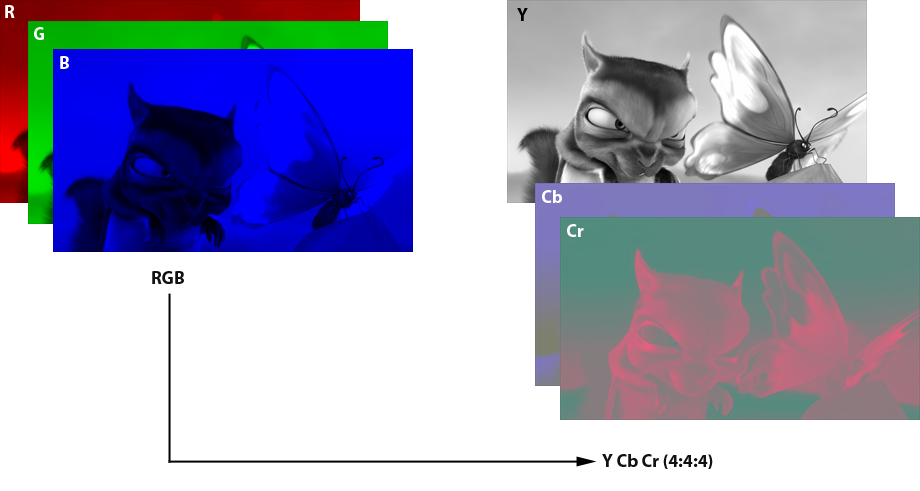
\includegraphics[width=0.75\textwidth]{Billeder/farvemodeller.png}
\caption{Eksempel på farvetransformation fra RGB til YCbCr [\citet{farvetransformation}, afsnit 4]}
\label{fig:farvemodeller}
\end{figure}
YCbCr står for \emph{Y}: Lysintensitet (en repræsentation af lysintensiteten i billedet), \emph{Cb} og \emph{Cr}: De to farverepræsentationer (hhv. blå minus \emph{Y} og rød minus \emph{Y}) [\citet{ycbcr_definition}, afsnit 1]. Fordelen ved YCbCr er at menneskets øje ikke opfatter forskelle i farver ligeså tydeligt som i lysintensitet, hvorved de to farverepræsentationer i højere grad kan komprimeres end lysintensiteten. Dette betyder at et billede i YCbCr-farverummet kan komprimeres mere end et i RGB-farverummet. Det skal dog bemærkes, at de to farverum udtrykker de samme data, blot med to forskellige baser. [\citet{ycbcr}, afsnit 2].

Der undersøges i følgende rapport med udgangspunkt i RGB-farverummet, da dette sparer transformationen til det nye farverum. Der ses bort fra, at brugen af YCbCr formentlig kunne have komprimeret billederne yderligere, men da forskelle på farverum ikke er fokus i denne rapport, bibeholdes billederne blot i RGB.
\begin{figure}[htbp]
\centering
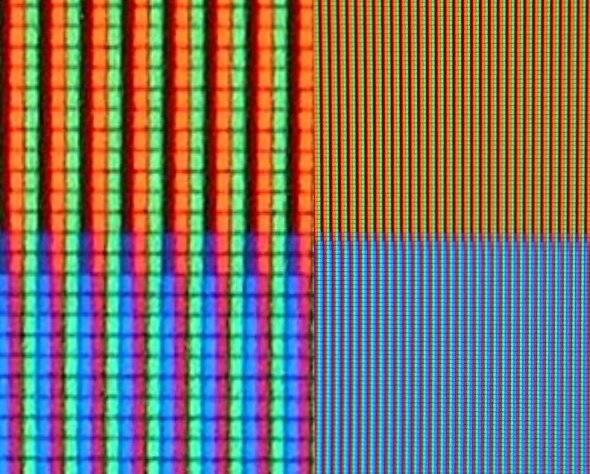
\includegraphics[width=0.35\textwidth]{Billeder/RGB_pixels.jpg}
\caption{Nærbillede af pixels, i farverne RGB.}
\label{fig:RGB_pixels}
\end{figure}

Når hver pixel kan beskrives ved én eller flere værdier, kan det digitale billede repræsenteres fuldstændigt som en matrix med indgange for hver pixels farveintensitet. Hvis billedet er et digitalt billede af dimensionerne $m \times n$, kan det altså beskrives ved en $m \times n$ matrix. Undersøges farvebilleder, transformeres de enkelte farver hver for sig. Et eksempel på et gråtonebillede ses på figur \vref{eq:pixelmatrix}.

\begin{figure}[htbp]
\begin{minipage}[b]{0.25\linewidth}
\centering

\includegraphics[width=\textwidth]{Billeder/8x8_blok2.png}
\caption{Billede af $8\times8$ pixels.}
\label{fig:pixelblok}
\end{minipage}
\hspace{0.5cm}
\begin{minipage}[b]{0.5\linewidth}
\centering
\[\begin{bmatrix}
5	&	176	&	193	&	168	&	168	&	170	&	167	&	165\\
6	&	176	&	158	&	172	&	162	&	177	&	168	&	151\\
5	&	167	&	172	&	232	&	158	&	61	&	145	&	214\\
33	&	179	&	169	&	174	&	5	&	5	&	135	&	178\\
8	&	104	&	180	&	178	&	172	&	197	&	188	&	169\\
63	&	5	&	102	&	101	&	160	&	142	&	133	&	139\\
51	&	47	&	63	&	5	&	180	&	191	&	165	&	5\\
49	&	53	&	43	&	5	&	184	&	170	&	168	&	74
\end{bmatrix}
\]
\caption{$8\times8$ matrix for billedet.}
\label{eq:pixelmatrix}
\end{minipage}
\end{figure}
Når digitale billeder kan repræsenteres af matricer, betyder det også, at de kan behandles ved brug af regneregler for matricer. Moderne billedbehandlingsteknikker udnytter regneregler for matricer, altså lineær algebra til at behandle digitale billeder.

Ud over at være i stand til at blive behandlet vha. lineær algebra har billeder den egenskab, at nærliggende pixels i et billede ofte udviser stor korrelation - de ligner hinanden og pixels kan derfor ofte beskrives ud fra de nærliggende pixels [\citet{lokminglui_DCT}, s. 4]. Dette udnyttes i den senere billedkomprimering.

\section{Billedkomprimering}
Billedkomprimering er en billedbehandlingsteknik, som søger at komprimere en billedfils størrelse. Billedkomprimeringsmetoder kan opdeles i to kategorier; \emph{tabsfri} og \emph{ikke-tabsfri} komprimering.

Mængden hvorved et billede kan komprimeres afhænger af mange faktorer, som bl.a. inkluderer billedets størrelse, om det er i gråtoner, sort/hvid eller farver, hvor mange forskellige farveintensiteter billedet indeholder, og hvilket format billedet er i. Som følge af disse faktorer er det ikke altid muligt at udvikle den ideelle metode, som kun fjerner ubetydelig information - nogle gange er det nødvendigt også at fjerne betydningsfuldt information.\\
Tabsfri betegner en komprimeringsteknik, som under komprimeringen ikke forårsager noget tab af information fra det originale billede. Her udnyttes det, at inputtet af informationer ikke er homogent, og at der derfor kan laves en statistisk model over disse informationer. Modellen bruges til at lave en komprimering eksempelvis ved brug af entropikodning, som vil blive forklaret nærmere i afsnit \vref{sec:Huffman}. Ved brug af tabsfri komprimering, er det dekomprimerede billede magen til det originale. Som følge af bevaringen af alle informationer af det originale billede, er det ikke altid muligt at lave effektive komprimeringer. Blandt tabsfri billedformater kan nævnes PNG og TIFF. Essensen i disse metoder er at de finder fordelagtige måder at udtrykke de samme data på.

Ikke-tabsfri komprimering betegner en komprimeringsteknik, som under komprimeringen forårsager uigenkaldeligt tab af informationer om det originale billede. Det dekomprimerede billede er en efterligning af det originale billede. Det er ikke helt magen til da informationerne, som er brugt til dekomprimering, ikke er identiske med informationerne om det originale billede. Komprimeringsteknikker med tab benytter det faktum, at nogle af informationerne om billedet er visuelt ligegyldige for det menneskelige øje. Som følge af dette kan et billedets kvalitet byttes for højere komprimeringsgrad, hvorved en større del betydelige informationer om det origninale billede tabes. Som følge af denne komprimeringstekniks større råderum i forhold til den tabsfri, kan denne også opnå langt større komprimeringsgrader end den tabsfri. Blandt billedformater med tab kan nævnes GIF og PNG [\citet{matthews}, afsnit 2 og 4].

Det udnyttes ofte i ikke-tabsfri komprimering, at nærliggende pixels i et billede har stor korrelation og derfor til en vis grad kan udtrykkes ved én samlet værdi i stedet for en værdi for hver enkelt pixel. Til dette bruges en transformation, som kan transformere et input med stor korrelation til et output uden stor korrelation, men som udtrykker korrelationen i det originale input [\citet{lokminglui_DCT}, s. 2 og 4]. I domænet med de ukorrellerede koefficienter, kan der derefter sorteres i koefficienterne for at bevare de, som er vigtigst for det samlede udtryk i det orginale input.